\documentclass{sciposter}
\usepackage[dvipsnames,usenames,svgnames,table,x11names, rgb, html]{xcolor} 
\usepackage{lipsum}
\usepackage{epsfig}
\usepackage{amsmath}
\usepackage{amssymb}
\usepackage[german]{babel}
\usepackage{geometry}
\usepackage{multicol}
\usepackage{graphicx}
\usepackage{tikz}
\usepackage{wrapfig}
\usepackage{gensymb}
\usepackage[utf8]{inputenc}
\usepackage{empheq}
\usepackage{mathpazo}
\usepackage[T1]{fontenc}
\renewcommand{\familydefault}{\rmdefault}
\usepackage{eulervm}

% for nice tableas
\usepackage{booktabs}

% so we have more space between matrix entries
\setlength{\arraycolsep}{12pt}

\geometry{
 landscape,
 a1paper,
 left=5mm,
 right=50mm,
 top=5mm,
 bottom=50mm,
 }


\usepackage{todonotes}

\newcommand{\nnz}{d\operatorname{nnz}}
\newcommand{\TODO}[1]{\todo[inline, color=red!40]{#1}}
\renewcommand{\vec}[1]{\mathbf{#1}}
%BEGIN LISTINGDEF



\usepackage{listings}
\usepackage{inconsolata}


\usepackage{mdframed}
\newenvironment{method}[1]{\begin{mdframed}[backgroundcolor=blue!10,innertopmargin=15pt, innerbottommargin=15pt, nobreak=true]
		\textbf{#1 }
	}
	{ 
	\end{mdframed}
}


\definecolor{background}{HTML}{FAFAFA}
\definecolor{comment}{HTML}{ABB0B6}
\definecolor{keywords}{HTML}{55B4D4}
\definecolor{basicStyle}{HTML}{6C7680}
\definecolor{variable}{HTML}{001080}
\definecolor{string}{HTML}{86B300}


\lstset{
	% How/what to match
	sensitive=true,
	% Border (above and below)
	frame=single,
	% Extra margin on line (align with paragraph)
	xleftmargin=\parindent,
	% Put extra space under caption
	belowcaptionskip=1\baselineskip,
	% Colors
	backgroundcolor=\color{background},
	basicstyle=\color{basicStyle}\ttfamily,
	keywordstyle=\color{keywords},
	commentstyle=\color{comment},
	stringstyle=\color{string},
	numberstyle=\color{sviolet},
	identifierstyle=\color{variable},
	% Break long lines into multiple lines?
	breaklines=true,
	% Show a character for spaces?
	showstringspaces=false,
	tabsize=2
}

%END LISTINGDEF


\newcommand*\widefbox[1]{\fbox{\hspace{2em}#1\hspace{2em}}}


\newlength\dlf  % Define a new measure, dlf
\newcommand\alignedbox[2]{
% Argument #1 = before & if there were no box (lhs)
% Argument #2 = after & if there were no box (rhs)
&  % Alignment sign of the line
{
\settowidth\dlf{$\displaystyle #1$}
    % The width of \dlf is the width of the lhs, with a displaystyle font
\addtolength\dlf{\fboxsep+\fboxrule}
    % Add to it the distance to the box, and the width of the line of the box
\hspace{-\dlf}
    % Move everything dlf units to the left, so that & #1 #2 is aligned under #1 & #2
\boxed{#1 #2}
    % Put a box around lhs and rhs
}
}
\usepackage{graphicx,url}

%BEGIN TITLE
\title{\huge{Numerical Methods for CSE}}

\author{\large{David Zollikofer}}
%END TITLE

\newcommand{\Q}{\mathbb{Q}}
\newcommand{\R}{\mathbb{R}}
\newcommand{\N}{\mathbb{N}}
\newcommand{\psection}[1]{\par \textbf{\large#1}}

\begin{document}
%\fontfamily{phv}\selectfont

\maketitle



\begin{multicols}{2}
	
\section*{Stuff I tend to forget}

\begin{itemize}
	\item \texttt{MatrixXd:Ones()} is not \texttt{MatrixXd::Identity()}
	\item Frobenius Norm ist die normale $\sqrt{\cdot}$ Norm mit dem Befehl \texttt{.norm()}.
\end{itemize}

\section*{\texttt{C++} Objects - Initializer Lists}



\begin{lstlisting}[language=c++]
class Point { 
	private: 
		int x; 
		int y; 
	public: 
		Point(int i = 0, int j = 0):x(i), y(j) {}  
			/*  The above use of Initializer list is optional as the  
			constructor can also be written as: 
			Point(int i = 0, int j = 0) { 
			x = i; 
			y = j; 
		} 
	*/    
}; 
\end{lstlisting}

\section*{Generics}

\psection{Functions and Generics}
\begin{lstlisting}[language=c++]
template <typename T> 
T mx(T x, T y){ 
	return (x > y) ? x : y; 
} 
int main() { 
	cout << mx<int>(3, 7) << mx<double>(3.0, 7.0) << mx<char>('g', 'e'); 
	return 0; 
} 

\end{lstlisting}

\psection{Classes and Generics}
\begin{lstlisting}[language=c++]
template <typename T, typename U> 
class A { 
	T x; 
	U y; 	
	public: 
		A() { cout << "constructor";} 
}; 
int main() { 
	A<char, char> a; 
	A<int, double> b; 
} 
\end{lstlisting}




\section*{Lambda Functions}
\psection{Lambda Functions \& Applying Coefficient wise}
\begin{lstlisting}[language=C++]
auto phi1 = [](int t) -> double {return 1/t;};
auto phi2 = [](int t){return 1/(t*t);};
b = b.unaryExpr(phi1);
\end{lstlisting}


\begin{lstlisting}[language=c++]
#include <functional>
int main(){
	std::function<double(int)>  f = [](int l){
		return l + 3.14;
	};
	std::cout << f(2);
}
\end{lstlisting}





\section*{Using \texttt{std::vector<...>}}


\psection{Turn \texttt{std::vector<...>} to \texttt{VectorXd}}

\begin{lstlisting}[language=c++]
std: :vector<double> t {12};
Map<VectorXd> te (t.data(),t.size());
\end{lstlisting}

\psection{General Usage}

\begin{lstlisting}[language=c++]
#include <vector>
std::vector<int> M {10,20,40,80,160,320,640,1280};
// Create a vector of size n with 
// all values as 10. 
vector<int> vect(n, 10); 
vector<int> g1; 
g1.push_back(123); 
g1.size(); 
g1.resize(4); 
g1.reserve(100);
cout << g1[2];
\end{lstlisting}



\section*{Using \texttt{std::pair<...,...>}}
\begin{lstlisting}[language=c++]
#include <utility>
std::pair<int, char> pr1; 
pr2 = make_pair("some text",4.56); 
pr1.first = 100; 
pr2.second = 'G' ; 
std::cout << pr1.first << " " << pr1.second ; 
\end{lstlisting}





\section*{Mathplotlib Plotting}

% matplotlibcpp
\begin{lstlisting}[language=c++]
// plotting results
plt::figure();
plt::plot(t, y, "+", {{"label", "approx IVP"}});
// exact solution 
VectorXd x = Vector::LinSpaced(100,0.0,T);
VectorXd exact = x.array().tan();
plt::plot(x, exact, {{"label", "tangent"}}  );
plt::legend();

plt::title("Approximate vs exact solution");
plt::xlabel("t");
plt::ylabel("y");
plt::grid("True");

plt::savefig("./cx_out/fileName.png");
\end{lstlisting}


\section*{Scientific Notation in C++}

The number \texttt{42030} can also be seen as \texttt{4.203e4} since we shift the decimal point 4 places to the left. Analogous with shifting to the right.
	
\section*{Constructing Matrices and Vectors}
\begin{lstlisting}[language=C++]
// same data different shape
Map<Matrix<TYPE, Dynamic , Dynamic>> newMat(M.data(),newRows,newCols);
// (Deep) copy data of M
MatrixXd xMat = MatrixXd::Map(M.data(), n, n);
\end{lstlisting}


\psection{Sizes, Rows, Cols, Resize}
\begin{lstlisting}[language=C++]
A.size() // total number of elements in matrix
A.rows() // number of rows
A.cols() // number of cols
A.resize(10,100) // resized to 10 rows and 100 columns
\end{lstlisting}


\psection{Filling matrices}
\begin{lstlisting}[language=C++]
A << R,	v // can also be done using blocks. 
u .transpose( ) ,  0;
B << A, A, A;     // B is three horizontally stacked A's.
A.fill(10);       // Fill A with all 10's.

MatrixXd::Identity(rows,cols)          
C.setIdentity(rows,cols)                 
MatrixXd::Zero(rows,cols)                
C.setZero(rows,cols)                      
MatrixXd::Ones(rows,cols)          
C.setOnes(rows,cols)                 
MatrixXd::Random(rows,cols)  // uniform random numbers in (-1,1).
C.setRandom(rows,cols)                 
VectorXd::LinSpaced(size,low,high)       // includes lower and higher bound -> if size=1 only higher. 
v.setLinSpaced(size,low,high)         
VectorXi::LinSpaced(((hi-low)/step)+1, low,low+step*(size-1))
\end{lstlisting}



\psection{Reshaping using Map}
\begin{lstlisting}[language=C++]
// same data different shape
Map<Matrix<TYPE, Dynamic , Dynamic>> newMat(M.data(),newRows,newCols);
// (Deep) copy data of M
MatrixXd xMat = MatrixXd::Map(M.data(), n, n);
\end{lstlisting}


\psection{Solving Equations}
\begin{lstlisting}[language=C++]
// Solve Ax = b. Result stored in x
x = A.ldlt().solve(b));  // A sym. p.s.d.    #include <Eigen/Cholesky>
x = A.llt().solve(b));  // A sym. p.d.      #include <Eigen/Cholesky>
x = A.lu().solve(b));  // Stable and fast. #include <Eigen/LU>
x = A.qr().solve(b));  // No pivoting.     #include <Eigen/QR>
x = A.svd().solve(b));  // Stable, slowest. #include <Eigen/SVD>
// .ldlt() -> .matrixL() and .matrixD()
// .llt()  -> .matrixL()
// .lu()   -> .matrixL() and .matrixU()
// .qr()   -> .matrixQ() and .matrixR()
// .svd()  -> .matrixU(), .singularValues(), and .matrixV()
\end{lstlisting}

\psection{Block}

Block of size (p,q), starting at (i,j) is \texttt{A.block(i,j,p,q);}


\psection{Triangular Views}
We have the following options \texttt{Upper, Lower, StrictlyUpper, StrictlyLower, UnitUpper, UnitLower}
\begin{lstlisting}[language=C++]
MatrixXd m2 = m.triangularView<Xxx>();
\end{lstlisting}

\psection{Diagonal}
\begin{lstlisting}[language=C++]
A = MatrixXd::Constant(n,n,0); // initialization is necessary
vec1 = mat1.diagonal();
mat1.diagonal() = vec1;
\end{lstlisting}

\psection{Reductions}
\begin{lstlisting}[language=C++]
R.minCoeff()              
R.maxCoeff()              
s = R.minCoeff(&r, &c)   
R.sum()                  
R.colwise().sum()      
R.prod()                
R.rowwise().prod()        
R.trace()                
(a > 2).all() // if all a_i > 2 true             
R.rowwise().all()     
(a > 2).any()    // if any a_i > 2 true        
(a > 2).count() // count a_i > 2 
R.colwise().any()  
x.norm()                 
x.squaredNorm()       
x.dot(y)                 
x.cross(y)     //Requires #include <Eigen/Geometry>
\end{lstlisting}




\TODO{sparse formats}
\TODO{CRS / COO format}




\TODO{timing 6.1 interpol -> see timing}


\psection{Kronecker Product}
\begin{lstlisting}
	C = kroneckerProduct(A,B).eval();
\end{lstlisting}


\section*{Sparse Matrices}

\psection{NNZ Arithmetics}
Es gilt:

\TODO{NNZ arithmetics}

\psection{Defining sparse matrices}
\begin{lstlisting}[language=C++]
#include <Eigen/Sparse>
SparseMatrix<double> mat(rows,cols);
std::vector<Triplet<double>> tripletVec;
tripletVec.reserve(n);
for(int i = 0; i < n; i++){
	double val = 2;
	Triplet<double> newTriplet(row,col,val);
	tripletVec.push_back(newTriplet);
}
X.setFromTriplets(tripletVec.begin(), tripletVec.end());
X.makeCompressed();
\end{lstlisting}



\psection{Solving Linear Equations with Sparse Matrices}
\begin{lstlisting}[language=C++]
Eigen::SparseMatrix<double> A(n,n);
A.reserve(3*n);
for(;;){
	A.insert(i,i-1) = 100;
}
A.makeCompressed(); // VERY IMPORTANT
Eigen::SparseLU<Eigen::SparseMatrix<double>> Ax_lu(A) 
newX = Ax_lu .solve(b);
\end{lstlisting}


\psection{Using sparse matrixes}
\begin{lstlisting}[language=c++]
	//now we loop over every non zero entry of M (for the left hand size of the kronecker product)
	// loop over every column
	for(int i = 0; i < n;i++){
		// we loop as long as there are still elements in the column
		// we get the pointer to where the column starts and loop for as long as elements still are in this column
		for(int index = colPointer[i]; index < colPointer[i+1] ; index++){
			// we are now at the nonzero element in row "i" and column "j" and value "outerValue".
			int outerRow = rowPointer[index];
			int outerColumn = i;
			double outerValue = values[index];
			
			// now we need to loop over all of M again to add the block to the kronecker matrix
			
			for(int innerI = 0; innerI < n;innerI++){
				// we loop as long as there are still elements in the row
				for(int innerIndex = colPointer[innerI]; innerIndex < colPointer[innerI+1] ; innerIndex++){
					
					int innerRow = rowPointer[innerIndex];
					int innerColumn = innerI;
					double innerValue = values[innerIndex];
					
					
					Triplet<double> toAdd(n*outerRow+innerRow,n*outerColumn+innerColumn,outerValue*innerValue);
					bVec.push_back(toAdd);
				}
			}
		}
	}
\end{lstlisting}

\section*{QR Decompositions}
\psection{Householder Reflection}
\begin{lstlisting}[language=matlab]
function [Q,R] = qr_householder(A)
%          Spiegelungen
%         R ... obere (upper) Dreiecks-Matrix
% Speicherplatz fuer Q & R
[m,n] = size(A);
Q = zeros(m,m);
R = zeros(m,n);
% Speicherplatz fuer die Householder-Spiegelungs Vektoren
U = zeros(m,n);
% QR-Zerlegung mit Householder-TransformationenBitte wenden!
R = A;
for j=1:n
% wir extrahieren die zu eliminierende spalte
w = R(j:m,j);
% falls m < n ist, breche bei hier ab wenn j > m
if ( j > m )
break
end
% waehle Spiegelung mit ?kleinster? Wirkung
if ( w(1) >= 0 )
w(1) = w(1) - norm(w);
else
w(1) = w(1) + norm(w);
end
% normiere Spiegelungs Vektor
u = w/(norm(w) + eps);
% speichere normierten Spieglungs Vektor in U% wende die Householder-Spiegelung auf A(j:m,j:n) an
U(j:m,j) = u; 
for i=j:n
R(j:m,i) = R(j:m,i) - 2.*u*(u'*R(j:m,i));
end
end% bauen nun Q? auf
Q = eye(m) - 2.*U(:,1)*U(:,1)';
for i=2:n
H = eye(m) - 2.*U(:,i)*U(:,i)';
Q = H*Q;
end
Q = Q';
\end{lstlisting}

\psection{Givens Rotation}
Grundlegende Idee. Wir killen alle Einträge unterhalb der Diagonale in $A$ und bauen uns $R$ draus.
$$\underbrace{\mathbb{1}G_1^{-1}\ldots G_k{-1}}_{=:Q} \underbrace{G_k \ldots G_1 A}_{=: R}$$
\begin{lstlisting}[language=matlab]
function [Q,R] = qrgivens(A)
	[m,n] = size(A);
	Q = eye(m);
	R = A;
	for j = 1:n
		for i = m:-1:(j+1)
			G = eye(m);
			[c,s] = givensrotation( R(i-1,j),R(i,j) );
			G([i-1, i],[i-1, i]) = [c, s; -s, c];
			R = G*R;
			Q = Q*G';
		end
	end
end
function [c,s] = givensrotation(a,b)
	if b == 0
		c = 1;
		s = 0;
	else
		if abs(b) > abs(a)
			r = a / b;
			s = 1 / sqrt(1 + r^2);
			c = s*r;
		else
			r = b / a;
			c = 1 / sqrt(1 + r^2);
			s = c*r;
		end
	end
end
\end{lstlisting}





\psection{Householder QR}
taken from code 3.3.3.29
\begin{lstlisting}[language=c++]
#include<Eigen/QR>
Eigen::HouseholderQR<MatrixXd> qr(A);
MatrixXd Q = qr.householderQ();
MatrixXd R = qr.matrixQR().template triangularView <Eigen::Upper>();
\end{lstlisting}


\section*{Least Squares}

\psection{Introduction}

We are interested in solving a problem $\vec{A} \vec{x} = \vec{b}$, where the system is overdeterminded, there might not exist a solution. We are aiming for $x \in \operatorname{argmin}\limits_{y\in \mathbb{K}^n} ||Ay - b||_2 ^2$.


\psection{Solve if $\vec{A}$ has full rank:}

We have two options:

\begin{itemize}
	\item \textbf{Normal Equation} $A^T Ax = A^T b$
	\begin{lstlisting}[language=c++]
	VectorXd x = (A.transpose()*A).llt().solve(A.transpose()*b);
	\end{lstlisting}
	\item \textbf{QR decomposition} $||Ax-b||_2 = ||Q(Rx - Q^H b)||_2 = ||Rx - Q^H b||_2$
	\begin{lstlisting}[language=c++]
	VectorXd x = A.householderQr().solve(b);
	\end{lstlisting}
\end{itemize}



\psection{Not full rank $\vec{A}$:}

We get infinitely many solutions if $\vec{A}$ doesn't have full rank. In this case we are interested in the 

\begin{mdframed}
	We define the \textbf{generalized solution} $x^+ := \operatorname{argmin}\{ ||x||_2 : x\in \operatorname{lsq}(A,b)\}$. Use Theorem 3.1.3.6 (Formula for generalized solution).
\end{mdframed}

For this we use the Singular Value Decomposition as seen in code 3.4.3.7 (Computing generalized solution of $Ax=b$ via SVD)


\begin{lstlisting}[language=c++]
JacobiSVD<MatrixXd> svd(A,ComputeThinU | ComputeThinV);
VectorXd solution = svd.solve(b);
\end{lstlisting}

\psection{Constrained Least Squares (3.6)}
Assume we want to minimize $|| Ax-b ||_2$ under the constraint $Cx = d$. We use Lagrangian multipliers and get the \textit{augmented normal equations}:
\begin{align*}
	  \begin{bmatrix}
	\vec{A}^T\vec{A} & \vec{C}^T \\ 
\vec{C} & 0 
	\end{bmatrix} \begin{bmatrix}
	\vec{x} \\ \vec{m} 
	\end{bmatrix} &= \begin{bmatrix}
	\vec{A}^T \vec{b}\\ \vec{d}
	\end{bmatrix}
\end{align*}
Alternatively we can also use the extended normal equations and get
\begin{align*}
\begin{bmatrix}
\vec{-I} & \vec{A} & 0\\
\vec{A}^T & 0 & \vec{C}^T\\
0 & \vec{C} & 0 
\end{bmatrix}
\begin{bmatrix}
\vec{r} \\ \vec{x} \\ \vec{m} 
\end{bmatrix} &=
\begin{bmatrix}
\vec{b}\\ 0 \\ \vec{d}
\end{bmatrix}
\end{align*}


\section*{Gaussian Block Elimination}
Example:\begin{align*}
\begin{bmatrix}
\vec{\mathbb{1}} & \vec{C^T} \\
\vec{C} & \vec{0}
\end{bmatrix} \cdot \begin{bmatrix}
\vec{x} \\ \vec{m}
\end{bmatrix} &= \begin{bmatrix}
\vec{0} \\ \vec{g}
\end{bmatrix}\\
\Rightarrow \vec{1\cdot x} + \vec{C^T\cdot m} &= \vec{0} \Rightarrow -\vec{C^T}\vec{m} = \vec{x}\\
\Rightarrow \vec{C x} &= \vec{g} \\
\Rightarrow \vec{-C}\cdot( \vec{C^Tm}) &= \vec{g}
\end{align*}



\section*{Data Interpolation and Fitting (Chapter 5)}


There are three main approaches:

\begin{itemize}
	\item Using Vandermonde Matrix $\rightarrow$ never do this. Very badly conditioned matrix.
	\item \textbf{Lagrange} Good choice, use Barycentric if interested in coeffs, if only need one eval use Aitken-Neville.
	\item \textbf{Newton} If we dynamically add new data (update friendly) (5.2.3.23)
\end{itemize}


\textbf{Extraplation to 0}: Works really well if $\phi(t) = \phi(-t)$, we use Aitken-Neville on extrapolation point.


\TODO{KONVERGENZ ZEUGS}




\section*{Function Approximation (Chapter 6)}

Approximation is the combination of an interpolation scheme and sampling. We get to choose where to evaluate the function $f$.

\begin{method}{Jackson's Theorem (6.1.1.11)}
	If $f\in C^r([-1,1])$ ($r\in \mathbb{N}$ times continuously differentiable), then for any polynomial of degree $n \geq r$
	\begin{align*}
		\inf_{p \in \mathcal{P}} || f-p ||_{L^\infty [(-1,1)]} \leq (1 + \frac{\pi^2}{2})^r \frac{(n-r)!}{n!} || f^{(r)} ||_{L^\infty [(-1,1)]}
	\end{align*}
\end{method}

We can also apply Jackson's Theorem to any interval using Lemma 6.1.1.20



\psection{Convergence}


\begin{itemize}
\item Algebraic Convergence: data on line in log-log plot, $\exists p > 0:$  $T(n) \leq n^{-p}$

\item Exponential Convergence: data on line in lin-log plot , $\exists 0 < q < 1:$  $T(n) \leq q^n$

\end{itemize}




\section*{Quadrature}


Basic Idea. We would like to calculate $\int_{a}^{b} f(x) dx = \sum_{j=1}^{n} w_j \cdot f(c_j)$, where $w_j$ are weights and $c_j$ are nodes. 

A \textit{Quadrature Rule} usually specifies weights and nodes on the interval $[-1,1]$, we then transform them accordingly to $[a,b]$

\begin{align*}
	w_i &\mapsto \frac{(b-a)}{2} \cdot w_i\\
	c_i &\mapsto \frac{1}{2}(1-c_i)a + \frac{1}{2}(1+c_i)b
\end{align*}

The \textbf{Quadrature Error} is given by $E_n(f) = \left| \int_{a}^b f(t) dt - Q_n(f)\right|$ 

\psection{Types of quadrature error}

\begin{itemize}
	\item \textsc{Algebraic Convergence} $E(n) = \mathcal{O}(n^{-p})$, $p > 0$
	\item \textsc{Exponential Convergence}  $E(n) = \mathcal{O}(q^n)$, $0 \leq q < 1$, here use \texttt{log} on the error and then do linear fitting.
\end{itemize}



\psection{Order of quadrature rules}

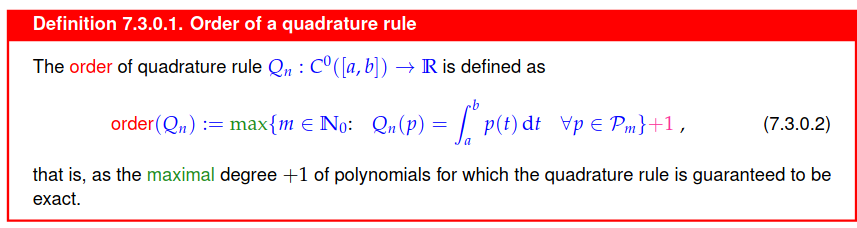
\includegraphics[width=\linewidth]{img/order.png}

Grundsätzlich: Newton-Cotes haben äquidistante Intervalle. Auf diesen Integrieren wir Lagrange Polynome, dies sind dann unsere Gewichte.

\TODO{make a small example}.


\begin{tabular}{|c|c|c|}
	\hline 
	$n$ &  & Order \\ 
	\hline 
	1 & midpoint rule & 2 \\ \hline 
	2 & trapezoidal rule & 2 \\ \hline 
	3 & simpson rule & 4 \\ \hline 
	4 & $\frac{3}{8}$-rule & 4 \\ \hline 
	5 & Milne rule & 6 \\ \hline 
	n & clenshaw curtis (from chebyshev, has all positive weights) & n \\ \hline 
	n & gauss legendre & 2n \\ \hline 
\end{tabular} 



\psection{Composite Quadrature}

Chop the integral into smaller integrals and integrate them seperately. Has algebraic convergence.


\psection{Order of Convergence}

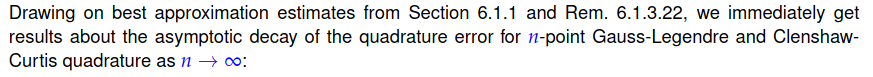
\includegraphics[width=\linewidth]{img/o1.png}
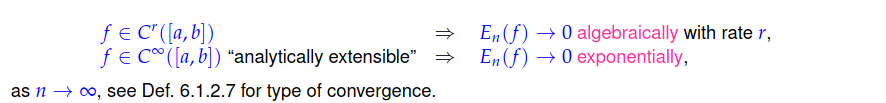
\includegraphics[width=\linewidth]{img/o2.png}




\section*{Differential Equations}

\psection{Transforming to autonomous 1st order ODE}

Assume we have $y'' = -g\sin(y)$, we define $u_1 = y$ and $u_2 = y'$. This yields:
\begin{align*}
	\vec{u} &= \begin{pmatrix}
	u_1 \\ u_2
	\end{pmatrix} = \begin{pmatrix}
	y \\ y'
	\end{pmatrix} & f(t,\vec{u}) = \begin{pmatrix}
	u_2 \\ -g\sin(u_1)
	\end{pmatrix} = \begin{pmatrix}
	u_1 '\\ u_2 '
	\end{pmatrix} = \vec{u}'
\end{align*}


We can also get rid of a dependence on $t$ (make autonomous): Assume we have $y' = -y + \cos(t)$. We define $v_1 = y$ and $v_2 = t$, this yields:
\begin{align*}
	\vec{v} &= \begin{pmatrix}
		v_1 \\ v_2
	\end{pmatrix} = \begin{pmatrix}
		y \\ t
	\end{pmatrix} & f(\vec{v}) = \begin{pmatrix}
		-v_1 + \cos(v_2) \\ 1
	\end{pmatrix} = \begin{pmatrix}
		v_1 '\\ v_2 '
	\end{pmatrix} = \vec{v}'
\end{align*}



\psection{Runge Kutta Methods}

We have the IVP  $\dot{\vec{y}} = \vec{f}(t,\vec{y})$, $\vec{y}(t_0) = \vec{y_0}$. We can write $\vec{y_1}$ as $$\vec{y}(t_1) = \vec{y_0} + \int_{t_0}^{t_1} \vec{f}(\tau, \vec{y}(\tau)) d\tau $$
giving us
$$
\vec{y}(t_1) \approx \vec{y_0} + h\sum_{i=1}^{s} b_i \vec{f}(t_0 + c_i h , \vec{y}(t_0 + c_i h))
$$

\psection{Butcher Scheme}
We call a single step Runge Kutta method consistent iff. 
\begin{align*}
	\begin{array}
	{c|c}
	\vec{c} &  \vec{A} \\
	\hline
	& \vec{b}^T
	\end{array} &:= 
	\begin{array}{c|cccc}
	c_1 &  0 & \ldots & \ldots & 0  \\
	c_2 &  a_{21} & \ddots &\ddots & \vdots\\
	\vdots & \vdots& \ddots & \ddots & \vdots \\
	c_s & a_{s1} & \ldots & a_{s,s_1} & 0\\
	\hline
	& b_1 &\ldots & \ldots b_{s-1} & b_s
	\end{array} 
\end{align*}

\psection{Find Order of Convergence of Runge-Kutta}
\begin{lstlisting}[language=c++]
VectorXd coeffs = polyfit(nArr.array().log(), err.array().log(),1); 
conv_rate = -coeffs(0);
\end{lstlisting}



\section*{Stiff Problems}

\psection{Calculating the stability function:}

The stability function $S(z)$ is defined as $y_1 = S(z)y(0)$ for any Runge-Kutta method.

\begin{itemize}
	\item \textbf{Explicit Euler} $y_1 = y_0 + h\cdot f(y_0)$, with model problem $y' = \lambda y$, hence we have $y_1 = y_0 + h\cdot \lambda \cdot y_0 = y_0 \left(1 + \lambda h\right) $. Using $z = h \lambda$ we get $S(z) = 1 + z$.
	\item \textbf{Trapezoidal rule} $y_1 = y_0 + h\frac{1}{2}(f(y_0) + f(y_0 + hf(y_0)))$ with $y' = \lambda y$, hence $y_1 = y_0 + h\frac{1}{2}(\lambda y_0 + \lambda y_0 + \lambda^2 h y_0)$ giving us $y_1 = y_0 + h\lambda y_0 + \frac{\lambda^2 h^2 y_0}{2}$ resulting in $y_1 = y_0 \left( 1 + h\lambda + \frac{\lambda^2 h^2}{2}\right)$ which yields the stability function $S(z) = 1 + z + \frac{z^2}{2}$.
\end{itemize}


\begin{method}{Stability Function via Butcher Table}
	The discrete evolution $\Psi_\lambda ^h$ of an $s$-stage Runge-Kutta single step method with Butcher scheme 	$\begin{array}
		{c|c}
		\vec{c} &  \vec{A} \\
		\hline
		& \vec{b}^T
	\end{array}$, the stability function is given by:
	$$S(z) = 1 + z\vec{b}^T(\vec{I} - z\vec{A})^{-1}\vec{1}$$
	where $\vec{1} = [1,\ldots,1]^T$
	
\end{method}

\begin{method}{Region of (absolute) Stability}
	$$S:\Phi := \{z \in \mathbb{C} : |S(z)| < 1  \} \subseteq \mathbb{C}$$
	This definition follows from the model problem $y' = \lambda y$ where we only have solutions that don't blow up if $|S(\lambda h)|<1$.
\end{method}

\begin{method}{Stiff Problems}
	A problem is stiff if it imposes much tighter timestep constraints (to keep the accuracy) on explicit single time step methods than the accuracy would usually require.
	
	An IVP for an autonomous ODE $\vec{y'} = \vec{f}(\vec{y})$ will probably be stiff, if, for substantial periods of time:
	$$\min\{\operatorname{Re} \lambda : \lambda \in \sigma (D\vec{f}(\vec{y}(t)))\} \ll 0$$
	where $t\to \vec{y}(t)$ is the trajectory and $\sigma$ is the set of eigenvalues. See example 12.2.0.16 for an example.
	
	Furthermore, if $\max\{\operatorname{Re} \lambda : \lambda \in \sigma (D\vec{f}(\vec{y}(t)))\} \approx 0$, we are unlikely to see blow ups.
\end{method}



\psection{Stability}

\begin{method}{A stability of RK method}
	A Runge-Kutta single step method with stability function $S$ is A-stable if
	$$\mathbb{C}^- := \{z \in \mathbb{C} : \operatorname{Re} Z < 0\} \subseteq S_\Phi$$
	where $S_\Phi$ is the stability region.
	
	Die Idee dahinter: Wenn die Testfunktion nicht explodiert $h\lambda = z \leq 0$, dann sollte das Verfahren für alle Zeitschritte nicht explodieren.
\end{method}

Nun gibt es aber das Problem, dass wir langfristig nicht explodieren aber grosse Diskretisierungsfehler haben. Um dies zu vermeiden gibt es:

\begin{method}{L stability of RK method}
	If the stability function $S(z)$ satisfies:
	$$\operatorname{Re} z < 0 \Rightarrow |S(z)| < 1$$
	$$\lim\limits_{\operatorname{Re}z \to - \infty} S(z) = 0$$
	
	Insbesondere gilt L-stabil $\iff$ A-stabil \& "$S(-\infty) = 0$"
\end{method}

Implicit Euler is L stable and Implicit midpoint is A stable.

\section*{Integrale Ausrechnen}


\subsection*{Direkte Integrale}
Diese sind vom Typ $\int f(g(x)) g'(x) dx = F(g(x))$.

\subsection*{Partielle Integration}
\begin{method}{Partielle Integration}
	\begin{align*}
	\int f' \cdot g \ dx = f \cdot g - \int f \cdot g' \  dx
	\end{align*}
\end{method}
\textbf{Beispiele}:


\subsection*{Integrale rationaler Funktionen}
\begin{method}{Partielle Integration}
	$$\int \frac{p(x)}{q(x)} dx$$
	Wenn nun $\deg(p) \geq \deg(q)$ dann machen wir eine Polynomdivision $p:q$, sonst mache eine Parzialbruchzerlegung
\end{method}

\subsection*{Substitutionsregel}
\begin{method}{Substitutionsregel}
	Ist $f$ stetig und $g$ erfüllt:
	\begin{align*}
	y = g(x) \iff x = g^{-1}(y)
	\end{align*}
	Dann gilt:
	\begin{align*}
	\int_a ^b f(g(x))g'(x) dx &= \int_{g(a)}^{g(b)} f(y) dy
	\end{align*}
	Als Merksatz gilt $dy = g'(x) dx$ respektive $dx = \frac{1}{t} dt$
\end{method}


\vfill\null
\columnbreak

% to have more vertical space in the table.

{\renewcommand{\arraystretch}{1.5}
	\begin{table}[]
		\begin{tabular}{@{} p{.25\textwidth} p{.3\textwidth} p{.45\textwidth} @{}}
			\toprule
			Funktion & Ableitung & Bemerkung / Regel\\ \midrule
			$x$ & $1$ &   \\
			$x^2$& $2x$ &   \\
			$x^n$& $n\cdot x^{n-1}$ & $n \in \R$  \\
			$\frac{1}{x} = x^{-1}$ & $- \frac{1}{x^2}$ & \\
			$\sqrt{x} = x^{\frac{1}{2}}$ & $\frac{1}{2\sqrt{x}}$ & \\ 
			$\sqrt[n]{x} = x^{\frac{1}{n}}$ & $\frac{x^{\frac{1}{n} -1 }}{n}$ &  $\int x^{1/n} dx = \frac{n x^{1/n + 1}}{n+1} + C$\\ 
			$e^x$ & $e^x$ & \\
			$a^x$ & $\ln(a) \cdot a^x$& \\
			$x^x = e^{x\log(x)}$ & $x^x \cdot (\log(x) + 1)$ & Kettenregel $e^{x\log(x)}$\\
			$\ln(x)$ & $\frac{1}{x}$ & \\
			$x\ln(x) - x$ & $\ln(x)$ &  \\ \midrule
			$\sin(x)$ & $\cos(x)$ & \\
			$\cos(x)$ & $- \sin(x)$ & \\ 
			$\tan(x) = \frac{\sin(x)}{\cos(x)}$ & $\frac{1}{\cos^2(x)} = 1 + \tan^2(x)$ &\\
			$\cot(x) = \frac{\cos(x)}{\sin(x)}$ & - $\frac{1}{\sin^2(x)}$ & \\ 
			$\arcsin(x)$ & $\frac{1}{\sqrt{1 - x^2}}$ & $ \arcsin : [-1,1] \to [-\frac{\pi}{2},\frac{\pi}{2}]$\\
			$\arccos(x)$ & $ - \frac{1}{\sqrt{1-x^2}}$ & $\arccos : [-1,1] \to [0, \pi]$\\
			$\arctan(x)$ & $\frac{1}{1+x^2}$ & $\arctan:(-\infty, \infty) \to (- \frac{\pi}{2},\frac{\pi}{2})$\\
			$\operatorname{arccot}(x)$ & $ - \frac{1}{1+x^2} $ & $\operatorname{arccot} : (-\infty, \infty) \to (0,\pi)$\\
			\midrule
			$\cosh(x)$ & $\sinh(x)$ &\\
			$\sinh(x)$ & $\cosh(x)$ & \\
			$\tanh(x)$ & $\frac{1}{\cosh^2(x)}$ & \\
			$\operatorname{arsinh}(x)$ & $\frac{1}{\sqrt{1+x^2}}$ & $\forall x \in R$\\
			$\operatorname{arcos}(x)$ & $\frac{1}{\sqrt{x^2 - 1}}$ & $\forall x \in (1, \infty)$\\		  $\operatorname{artanh}(x)$ & $\frac{1}{1-x^2}$ & $\forall x \in (-1,1)$\\
			\midrule
			$g(x) \cdot h(x)$ & $g(x) \cdot h'(x) + g'(x) \cdot h(x)$ & Produktregel\\
			$\left(g(x)\right)^n$ & $n \cdot \left( g(x) \right)^{n-1} \cdot g'(x)$ & Potenzregel\\
			$\frac{g(x)}{h(x)}$ & $\frac{ g'(x) \cdot h(x) - g(x)\cdot h'(x)}{\left(h(x)\right) ^2}$ & Quotientenregel\\
			$h(g(x))$ & $h'(g(x)) \cdot g'(x)$ & Kettenregel\\
			\bottomrule
		\end{tabular}
	\end{table}
}

\vfill\null
\columnbreak



\end{multicols}
\end{document}